\section{Altri tipi di alberi}
\subsection{Alberi perfettamente bilanciati}
Un albero è \emph{perfettamente bilanciato} quando per ogni nodo la differenza tra il 
numero di nodi del sottoalbero sinistro e il numero di nodi del sottoalbero destro
è al massimo 1.
\subsection{Alberi bilanciati in altezza o AVL}
Un albero è \emph{bilanciato in altezza} o \emph{AVL} quando per ogni nodo la differenza
in valore assoluto tra l'altezza del sottoalbero destro e l'altezza del sottoalbero sinistro è
al massimo 1.\\
\textbf{N.B} bilanciato in altezza $\Rightarrow$ bilanciato, ma non viceversa.\\
\textbf{Numero massimo di nodi}: $2^{h+1} - 1$\\[20pt]
\textbf{Numero minimo di nodi}:
\begin{equation*}
    \begin{cases}
        1 & \text{se h = 0}\\
        2 & \text{se h = 1}\\
        1 + n_{h-1}+n_{h-2} & \text{se h $>$ 1}
    \end{cases}
\end{equation*}
\begin{wrapfigure}{r}{7cm}
    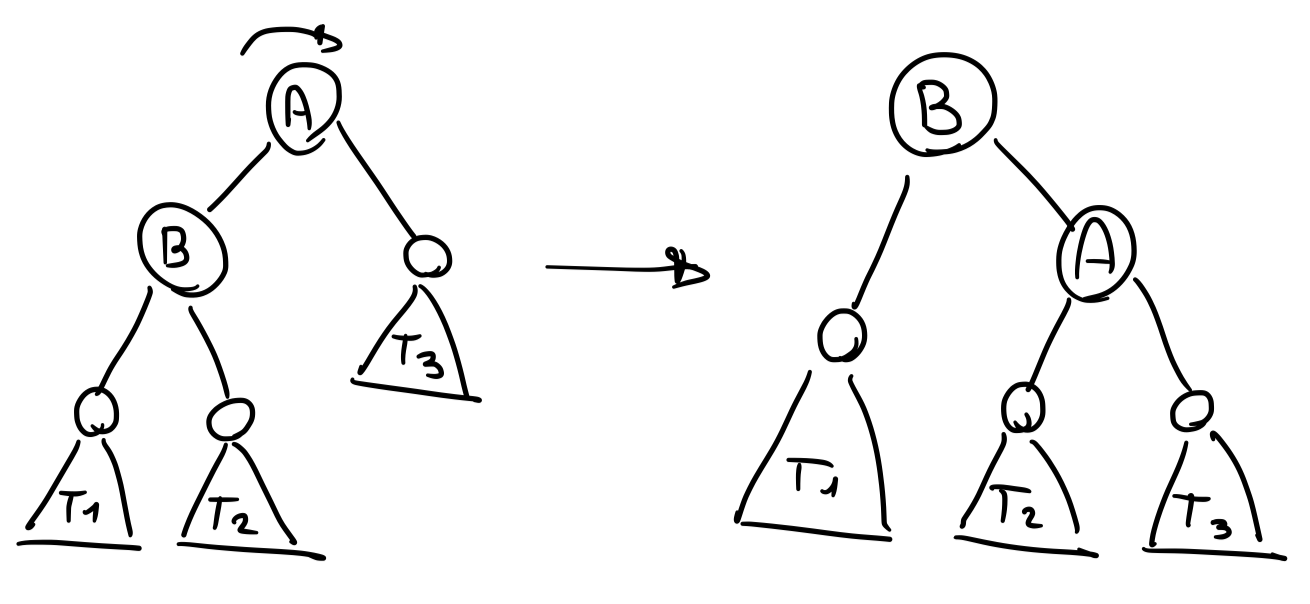
\includegraphics[scale = 0.3]{albero_sbilanciato.png}
\end{wrapfigure}
Un albero AVL con il minimo numero di nodi è detto \emph{albero di Fibonacci}
Nel caso l'albero risulti sbilanciato devo eseguire delle operazioni per sistemarlo.

\subsubsection*{Costo operazioni}
Dato un albero di ricerca di $n$ nodi
\begin{itemize}
    \item Ricerca $O(\log_2 n)$
    \item Inserimento $O(\log_2 n)$
    \item Cancellazione $O(\log_2 n)$
\end{itemize}

\noindent Questa per ora è la struttura con prestazioni migliori per i dizionari, almeno 
finchè non vedremo le tabelle hash più avanti.

\subsection{Alberi 2-3}
Gli \emph{alberi 2-3} sono alberi in cui ogni nodo interno ha 2 o 3 figli
e le foglie sono tutte allo stesso livello. I dati sono memorizzati solo nelle foglie
e i nodi interni contengono solo informazioni di instradamento.
\begin{itemize}
    \item Se la chiave di un nodo interno contiene solo un valore, significa che il nodo ha 2 figli,
        e quel valore è il maggiore del sottoalbero sinistro
    \item Se la la chiave di un nodo interno contiene 2 valori significa che il nodo ha 3 figli, e i due
    valori corrispondono rispettivamente al massimo valore contenuto nel sottoalbero sinistro e al massimo
    valore contenuto nel sottoalbero centrale
\end{itemize} 
    
\begin{figure}[h]
    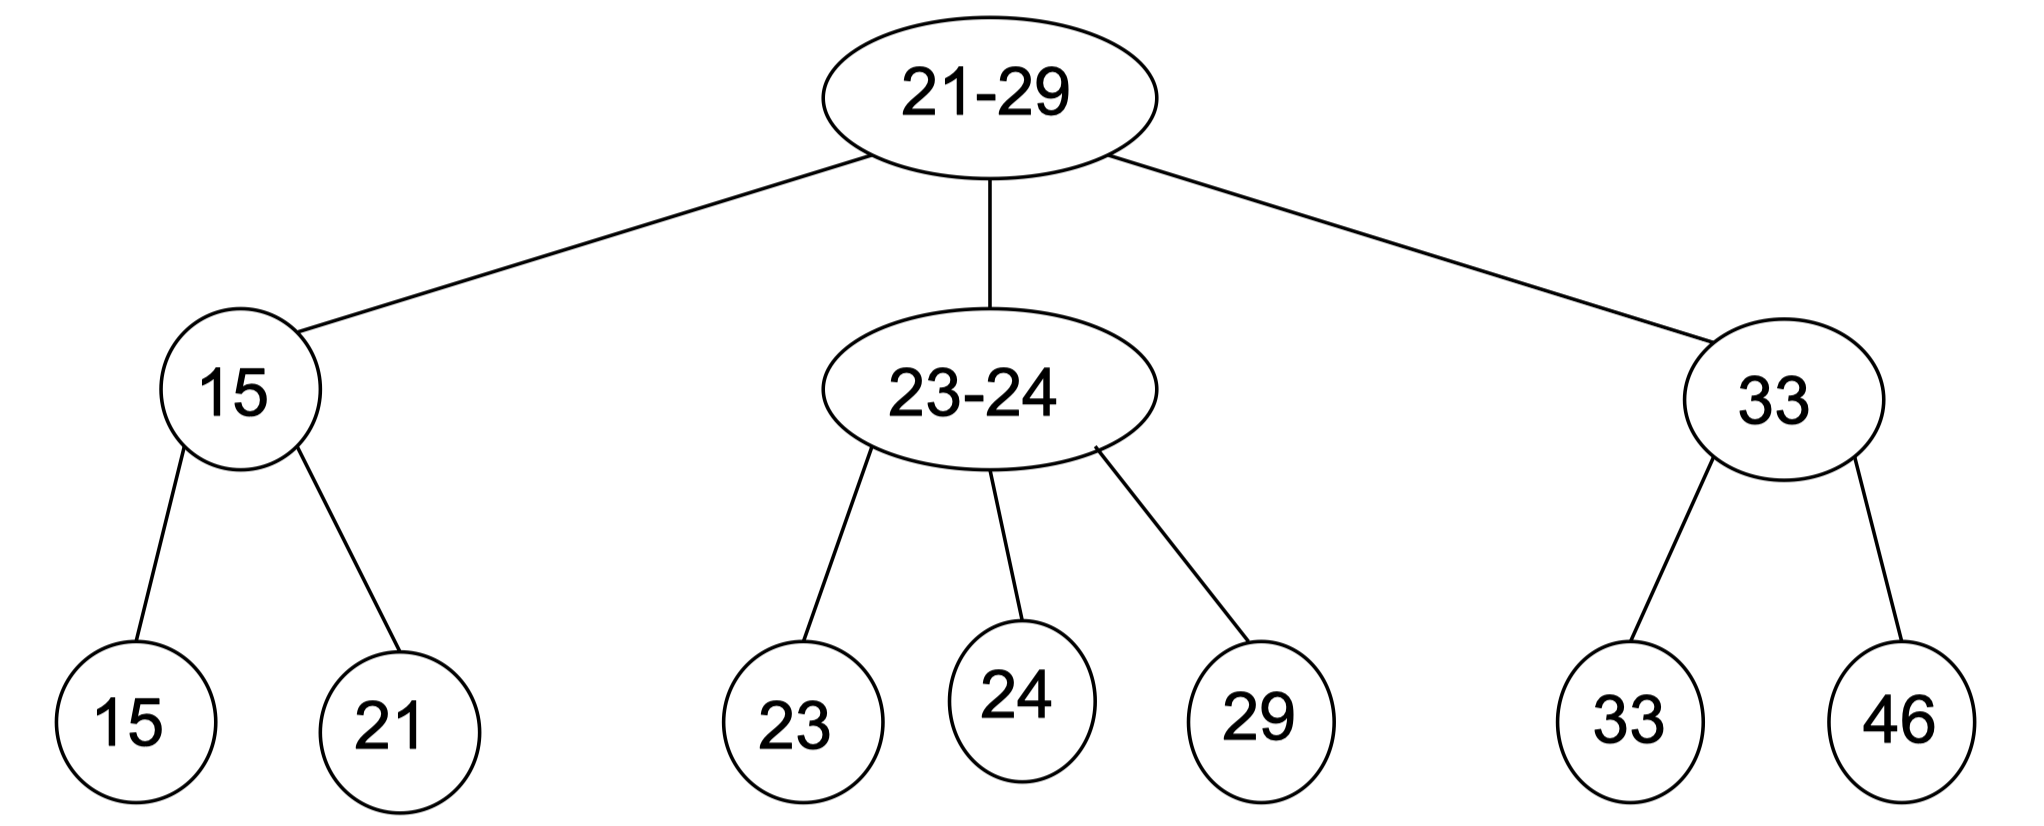
\includegraphics[width = \textwidth]{albero_2-3.png}
\end{figure}

\begin{tabular}{|l|c|c|}
    \hline
    \space & \textbf{min} & \textbf{max}\\
    \hline
    \textbf{Numero nodi} & $2^{h+1}-1$ & $\frac{3^{h+1}-1}{2}$\\
    \hline
    \textbf{Numero foglie} & $2^{h}$ & $3^{h}$\\
    \hline
\end{tabular}
\subsubsection{Operazioni}

\begin{algorithm}
    \caption{Ricerca di un dato}
    \Indm\textbf{Funzione} \emph{trova(albero2-3 r, tipoChiave k)} $\rightarrow$ \emph{foglia}\\
    \Indp$n \leftarrow r$\\
    \While{n si riferisce ad un nodo interno}{
        \eIf{$k \le n.s$}{$n \leftarrow n.sx$}{$n \leftarrow n.dx$}
    }
    \eIf{$n.chiave = k$}{ \Return $n$}{\Return{null}}
\end{algorithm}

\noindent Per inserimenti e cancellazioni è utile tenere in ogni nodo un puntatore al nodo padre.
Quando un nodo ha già 3 figli e devo inserirne un altro, faccio uno \emph{split}.
\clearpage
\begin{figure}[h]
    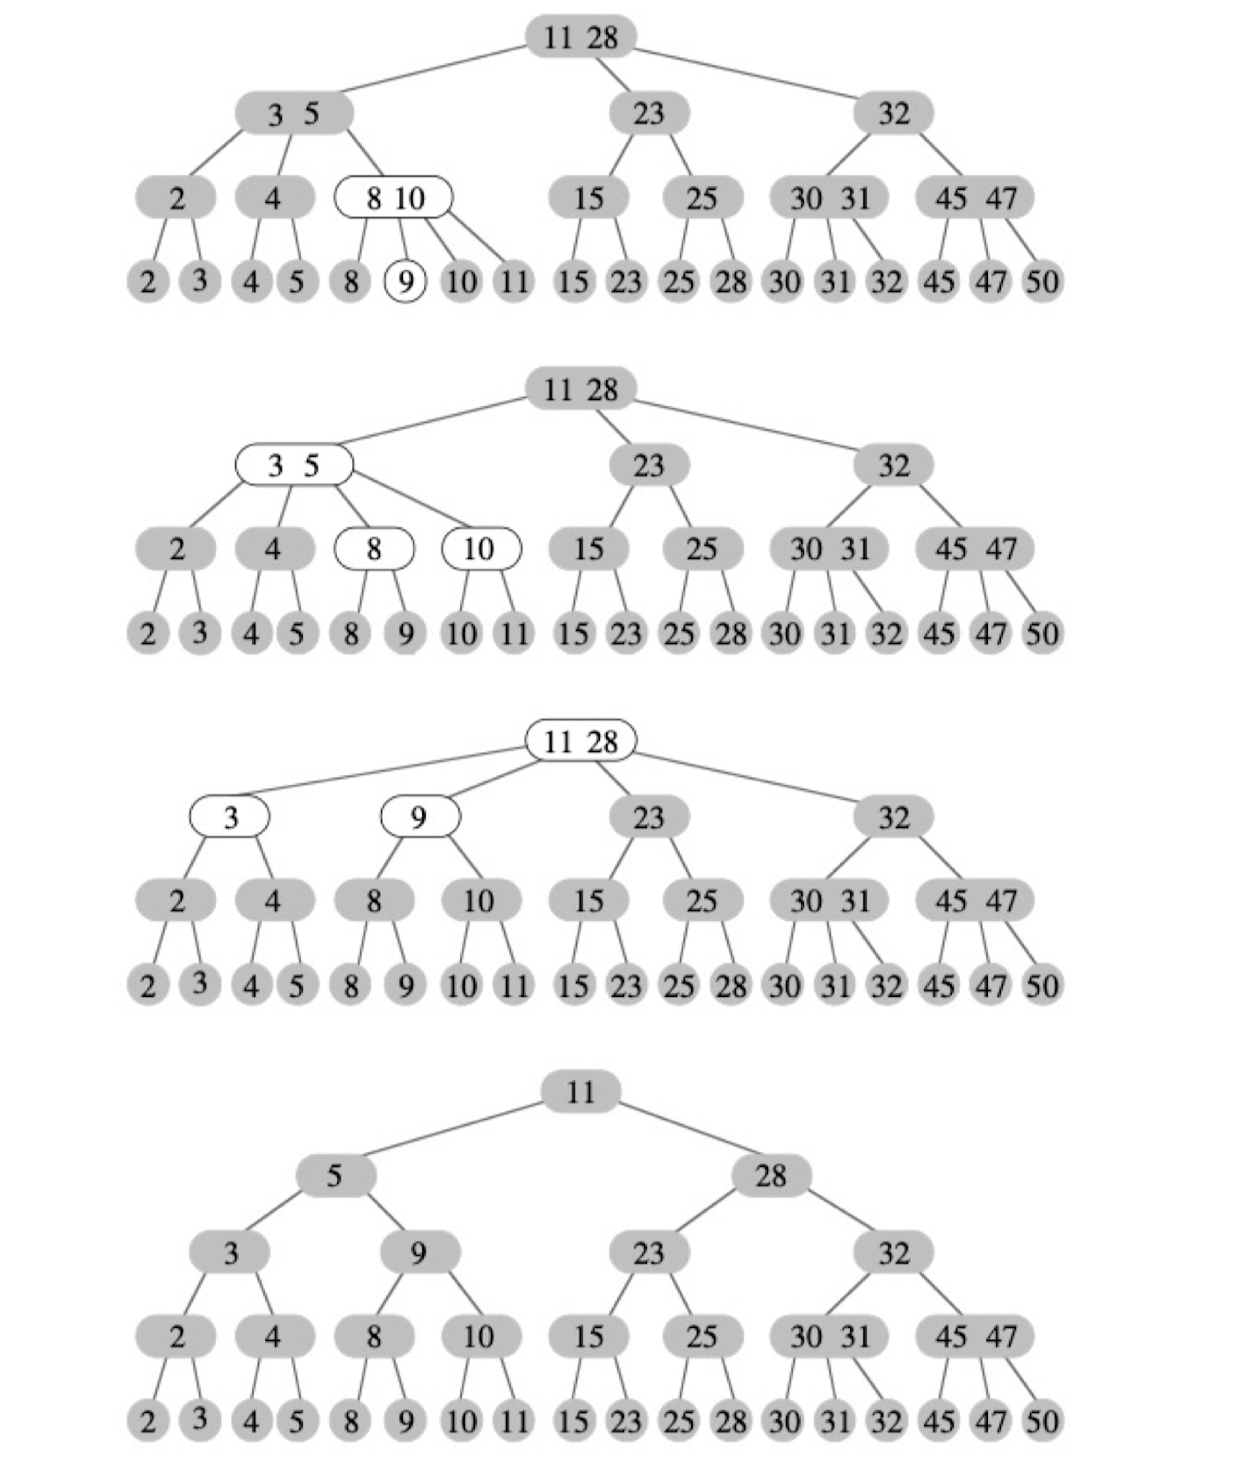
\includegraphics[width=\textwidth]{albero_2-3_split.png}
\end{figure}
\clearpage
\subsubsection{Costo operazioni}
\begin{itemize}
    \item \textbf{Ricerca}: $O(\log n)$
    \item \textbf{Inserimento}: $O(\log n)$
    \item \textbf{Cancellazione}: $O(\log n)$
\end{itemize}
Come gli alberi AVL.
\subsection{B-Alberi}
Sono un modello nato per rappresentare gli indici delle basi di dati, quando i 
dati sono troppo grandi per stare in memoria centrale. L'obiettivo non è più 
quello di fare l'albero più basso possibile, ma quello di fare il minor numero possibile di 
accessi al disco. A differenza degli alberi 2-3 le informazioni non sono solo nelle foglie
ma anche nei nodi interni.
Diamo una definizione formale di \emph{B-albero} di ordine $t$ (dove $t$) è il grado minimo:
\begin{itemize}
    \item Ogni nodo interno ha al massimo $2t$ figli 
    \item Ogni nodo interno diverso dalla radice ha almeno $t$ figli 
    \item La radice ha almeno 2 figli
    \item Tutte le foglie hanno la stessa profondità 
    \item Ogni foglia contiene $k$ chiavi ordinate dove $t - 1 \le k \le 2t - 1$
    \item Ogni nodo interno con $k + 1$ figli e sottoalberi $T_0...T_k$ contiene 
    $k$ chiavi ordinate tali che per ogni chiave $c_i$ nell'albero $T_i$ (con $i=0...k$) si ha:
    \begin{center}
        $c_0 \le a_1 \le c_1 \le a_2 \le ... \le a_{k-1} \le c_{k-1} \le a_k \le c_k$
    \end{center}
\end{itemize}
\noindent \textbf{Numero minimo di chiavi in un albero di altezza $h$}: $2t^{h}-1$\\
\textbf{Altezza massima $n$ chiavi}: $2t^{h}-1$\\
\textbf{Passi totali ricerca}: $\Theta(h \cdot \log t)$\\

\subsubsection*{Costo operazioni}

\begin{tabular}{|l|c|c|}
    \hline
    \space & \textbf{Passi di calcolo(tempo)} & \textbf{Accessi a memoria di massa}\\
    \hline
    \textbf{Ricerca} & $\Theta(\log n)$ & $\log_t n$\\
    \hline
    \textbf{Inserimento} & $\Theta(t \cdot \log n)$ & $c \cdot \log_t n$\\
    \hline
    \textbf{Cancellazione} & $\Theta(t \cdot \log n)$ & $c \cdot \log_t n$\\
    \hline
\end{tabular}
\begin{itemize}
    \item $n$ = numero di chiavi
    \item $c$ = costante piccola (dipende dall'implementazione, di solito è circa 4)
\end{itemize}

\clearpage


